\section{The \ourmethod System Architecture}
\label{sec:architecture}

\ourmethod has three components that run as a pipeline.
First, the \emph{Column Profiler} reads the data once and summarizes every column.
Second, the \emph{Ring Builder} turns these summaries into candidate key domains, called rings, without any LLM call.
Third, the \emph{Budgeted Verifier} decides which candidates need the LLM, verifies each ring with one batched prompt, and returns the join graph.
Only the third component calls the LLM.
Figure~\ref{fig:system_arch} shows the three components and the data that flows between them.

\begin{figure*}[t]
    \centering
    \resizebox{\textwidth}{!}{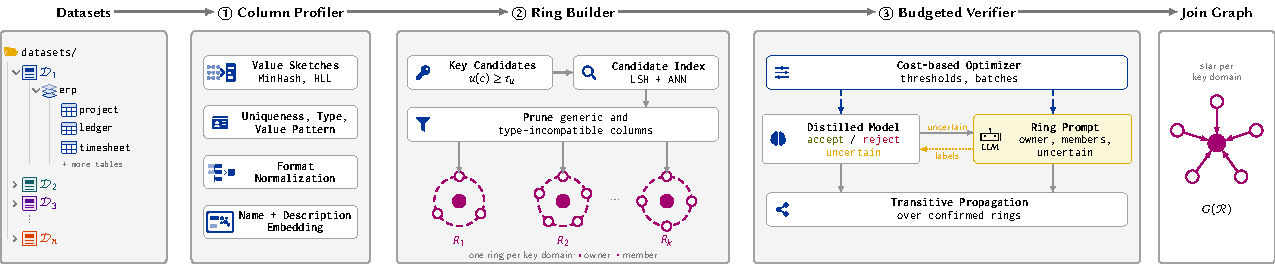
\includegraphics{figures/img/fig_KeyRing_Architecture}}
    \caption{\ourmethod architecture: the \textbf{Column Profiler} summarizes every column in one pass without the LLM; the \textbf{Ring Builder} groups candidate key columns into rings, one per key domain, each with an owner; the \textbf{Budgeted Verifier} accepts or rejects confident candidates with a distilled model, verifies each ring with one batched LLM prompt, and propagates joins by transitivity, so that the join graph keeps a target recall of the all-pairs LLM baseline.}
    \label{fig:system_arch}
\end{figure*}

\introparagraph{Design Principles}
Three principles shape \ourmethod, each serving requirements from Section~\ref{sec:problem}.
First, \ourmethod decides key domains, not table pairs.
The LLM verifies a ring once, and the joins of all its members follow from that answer, so the number of LLM calls grows with the number of key domains (R2), and the output is a star around each owner (R4).
Second, \ourmethod uses each signal for what it is reliable at.
Uniqueness, containment, and embeddings are reliable for proposing candidates, but not for deciding what a column means.
The Ring Builder therefore tunes them for recall, because a join it drops cannot be recovered later, and leaves meaning to the LLM.
Third, \ourmethod pays for the LLM only where its answer changes the outcome, and it reuses every answer it pays for.
A local model, trained only on \ourmethod's own LLM answers, decides confident candidates (R3), and a cost-based optimizer sets its thresholds so that the result meets the recall target (R1).

\subsection{Column Profiler}
\label{sec:arch_profiler}
The Column Profiler makes one pass over the data and computes a profile for each column $c \in \mathcal{C}$.
The profile has four parts, shown on the left of Figure~\ref{fig:system_arch}.
First, \emph{value sketches}: a MinHash sketch of the distinct values for containment estimates~\cite{DBLP:journals/pvldb/ZhuNPM16}, and a HyperLogLog sketch for the number of distinct values.
Second, \emph{statistics}: the uniqueness $u(c)$, the null ratio, the data type, and a value pattern, such as ``three letters, a dash, and five digits''.
Third, \emph{normalized formats}: the profiler strips leading zeros, prefixes, and case differences, and sketches the normalized values as well, so that a join with zero exact overlap can still show containment.
Fourth, an \emph{embedding} of the column name together with its LLM annotation, if the annotation step of the current pipeline (Section~\ref{sec:bg_llm}) has already produced one.
The cost of profiling is linear in the size of the data, and no later step reads raw data again.

\subsection{Ring Builder}
\label{sec:arch_ringbuilder}
The Ring Builder turns profiles into rings in four steps, shown in the middle of Figure~\ref{fig:system_arch}.
First, it selects \emph{key candidates}: columns with uniqueness $u(c) \geq \tau_u$ and few nulls, which can own a key domain.
Second, it generates \emph{candidate references} for every column with two indexes over the key candidates: a containment index on the value sketches~\cite{DBLP:journals/pvldb/ZhuNPM16}, and an approximate nearest-neighbor index on the embeddings.
The first index finds references with overlapping values, and the second finds references whose values differ in format but whose names and descriptions match.
Third, it \emph{prunes} candidates that cannot be keys: columns whose type is incompatible with the owner, and generic columns, such as \texttt{DATA} or small status codes, that match a large fraction of all key candidates.
Fourth, it \emph{forms rings}.
Each key candidate with at least one remaining reference starts a ring, and each referencing column joins the ring of its best-scoring owner.
When two owners reference each other, such as a master table and its staging copy, the Ring Builder merges their rings and elects the owner with the larger domain.
The output is a set of candidate rings, each with an owner, its members, and a score for each member.
Section~\ref{sec:ring_builder} describes these steps in detail.

\subsection{Budgeted Verifier}
\label{sec:arch_verifier}
The Budgeted Verifier turns candidate rings into confirmed rings in four steps, shown on the right of Figure~\ref{fig:system_arch}.
First, the \emph{cost-based optimizer} draws a random sample of candidates and asks the LLM about them.
From these answers, it sets two thresholds on the score of the distilled model, so that the result keeps a target recall $\gamma$ of the oracle with probability at least $1-\delta$, in the style of SUPG and BARGAIN~\cite{SUPG,BARGAIN}.
It also chooses how many candidates to place in one prompt.
Second, the \emph{distilled model} scores every remaining candidate from its profile features.
It accepts candidates above the upper threshold and rejects candidates below the lower threshold.
Third, the \emph{ring prompt} verifies each ring that still has uncertain members.
One prompt contains the owner, the accepted members, and the uncertain candidates of a ring, and the LLM confirms the owner and returns the members that refer to it.
Every LLM answer becomes a label, so the distilled model improves while the verifier runs.
Fourth, \emph{transitive propagation} derives the remaining joins: every confirmed member joins its owner, and two members of the same ring join through it.
The output is the join graph $G(\mathcal{R})$ of Section~\ref{sec:problem}.
Section~\ref{sec:verifier} describes the optimizer and its guarantee.

\begin{example}[Running Example]
In the services firm of Section~\ref{sec:introduction}, the profiler computes the profile of the project master's \texttt{PROJECT\_CODE}, which is unique, and of the $k$ columns that reference it.
Normalization removes the leading zeros of the padded export, so its codes are contained in the master again.
The containment index proposes \texttt{PRJ\_ID} and the padded column as references, and the embedding index proposes \texttt{ENGAGEMENT}, whose values carry a prefix.
The Ring Builder prunes \texttt{DATA}, which matches \todo{X}\% of all key candidates, and merges the staging copy of the master into the same ring.
The distilled model accepts the confident members and rejects the surrogate \texttt{ID} columns, whose values are contained in the codes by accident.
The LLM then verifies the ring with a single prompt that lists the uncertain members, instead of answering $\binom{k+1}{2}$ pairwise prompts.
\end{example}

\section{Column Profiling and Ring Building}
\label{sec:ring_builder}
\todo{Key candidate selection, the two candidate indexes, pruning of generic columns, ring formation and owner election, complexity.}

\section{Budgeted Verification}
\label{sec:verifier}
\todo{Distilled model, threshold selection with recall guarantee, ring prompts and batching, transitive propagation, cost analysis.}
